\documentclass{article}

\usepackage{graphicx}

\title{Lab 5}
\author{Filip Jędrzejewski}

\begin{document}
	\maketitle
	
	\section*{Zadanie 1}
	
	\subsection*{Opis problemu}
	
	Celem zadania było wykonanie aproksymacji średniokwadratowej punktowej populacji Stanów Zjednoczonych wielomianami stopnia $m$ ($0 \leq m \leq 6$) dla danych:
	
	\begin{center}
		\begin{tabular}{c|c}
  			\hline 
  			Rok & Populacja\\
  			\hline
  			1900 & 76 212 168 \\
  			1910 & 92 228 496 \\
  			1920 & 106 021 537 \\
  			1930 & 123 202 624 \\
  			1940 & 132 164 569 \\
  			1950 & 151 325 798 \\
  			1960 & 179 323 175 \\
  			1970 & 203 302 031 \\
  			1980 & 226 542 199 \\
		\end{tabular} 
		
	\end{center}	
	
	\subsection*{Ekstrapolacja do roku 1990}
	
	Wielomian wyznaczano za pomocą funkcji \texttt{numpy.polynomial.polynomial.Polynomial.fit()}. Dla każdego wielomianu dokonano jego ekstrapolacji do roku $1990$ i porównywano jego wartość z wartością prawdziwą wynoszącą $248 709 873$. Wyniki błedu względnego dla każdego wielomianu przedstawiono w tabeli:
	
	
	\begin{center}
		\begin{tabular}{c|c}
  			\hline 
  			Stopień wielomianu & Błąd względny\\
  			\hline
  			$0$ & $0,4235$ \\
  			$1$ & $0,0519$ \\
  			$2$ & $0,0241$ \\
  			$3$ & $0,0512$ \\
  			$4$ & $0,0225$ \\
  			$5$ & $0,1137$ \\
  			$6$ & $0,0255$ \\
		\end{tabular} 
		
	\end{center}	
	
	Najmniejszym błędem obarczony był wielomian stopnia 4. \\
	
	\subsection*{Wykres}	
	
	Aproksymowane wielomiany, dane wejściowe i prawdziwa wartość dla $1990$ roku zostały przedstawione na wykresie:
	
	
	\begin{figure}[h]
    		\centering
  		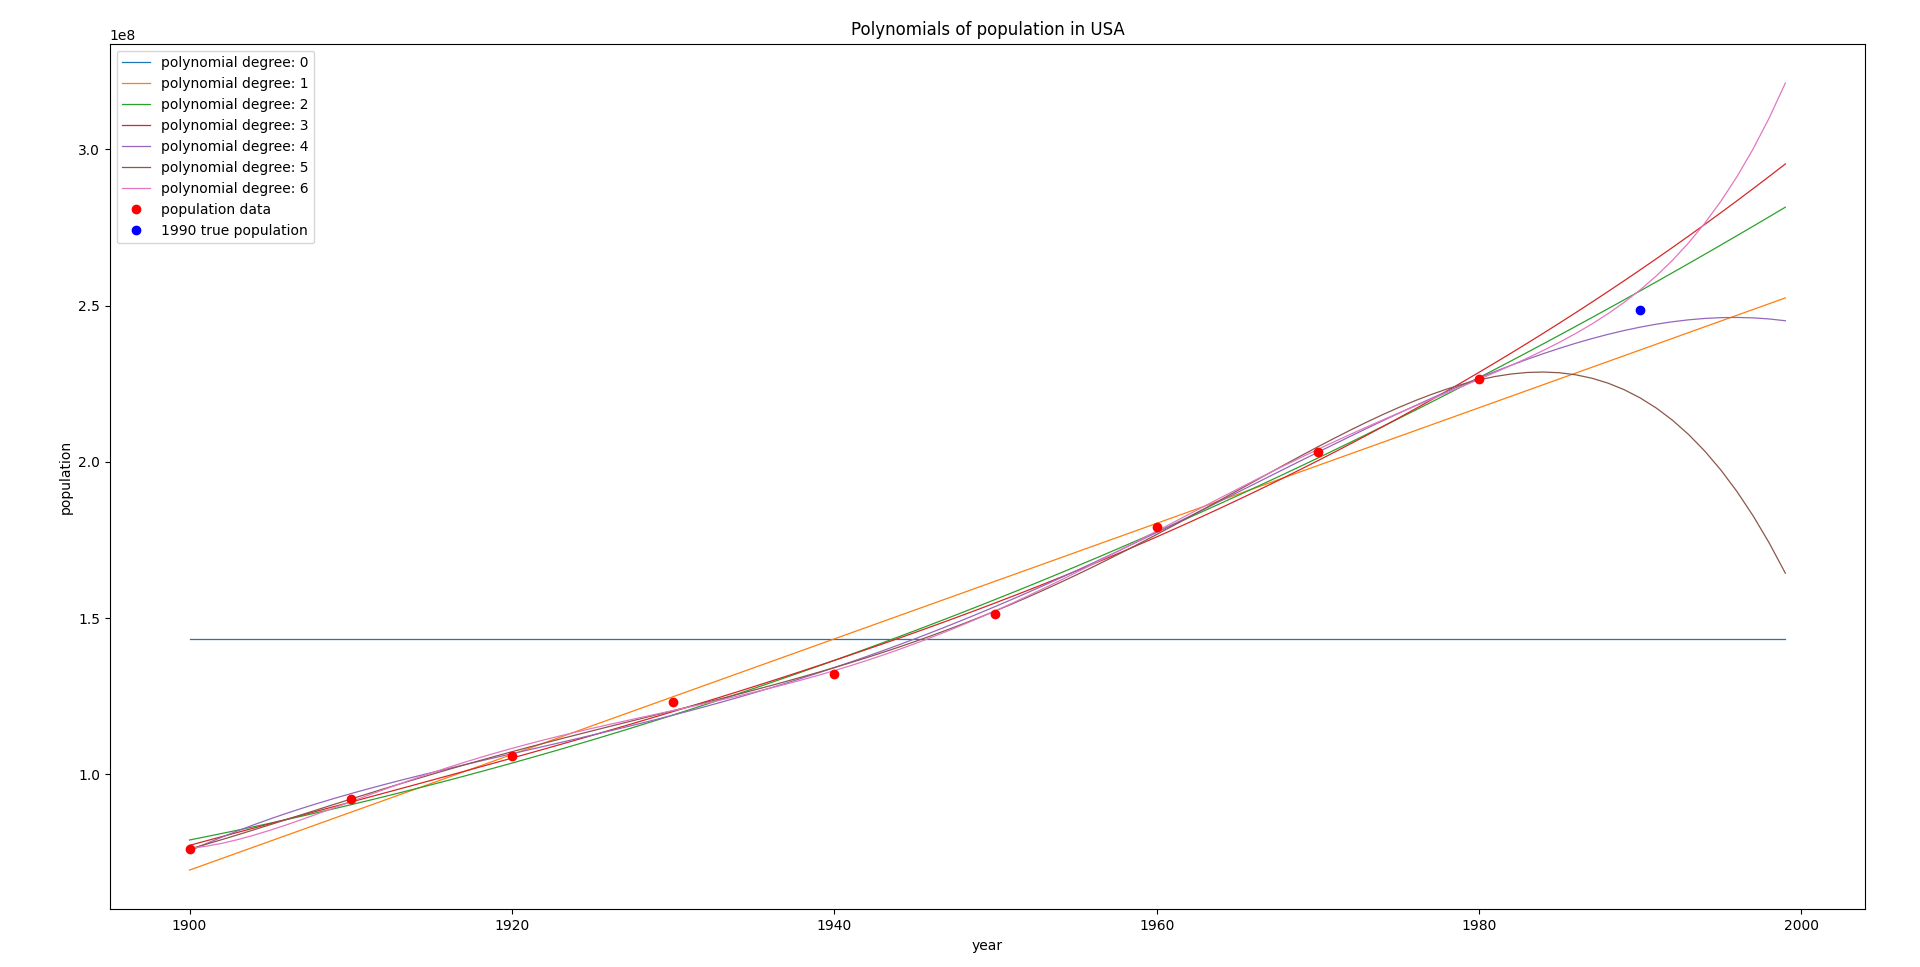
\includegraphics[scale = 0.3]{wykres1.png}
	\end{figure}
	
	\subsection*{Kryterium informacyjne Akaikego}
	
	W celu znalezienia najlepszego stopnia wielomianu aproksymującego dane, można się posłużyć kryterium informacyjnym Akaikego:
	
	\begin{equation}
		AIC = 2k - k \ln \left( \frac{\sum^n_{i=1} [y_i - \^y (x_i)]^2}{k} \right)
	\end{equation}
	
	gdzie: $k = m+1$, $y_i$ - prawdziwa wartość funkcji dla argumentu $x_i$, $\^y (x_i)$ - wartość funkcji przewidywana przez model (wartośc wielomianu dla argumentu $x_i$). Jeżeli rozmiar próbki ($n$) jest niewielki, czyli $\frac{n}{k} < 40$, to należy dodać do wzoru (1) składnik korygujący:
	
	\begin{equation}
		AIC = AIC + \frac{2k(k+1)}{n-k-1}
	\end{equation}
	
	\newpage	
	
	Im wartość AIC jest mniejsza, tym model jest lepszy. Obliczone wartości AIC dla wyznaczonych wielomianów zapisano w tabeli:
	
	\begin{center}
		\begin{tabular}{c|c}
  			\hline 
  			Stopień wielomianu & AIC\\
  			\hline
  			$0$ & $-35.01$ \\
  			$1$ & $-59.91$ \\
  			$2$ & $-82.05$ \\
  			$3$ & $-103.86$ \\
  			$4$ & $-117.90$ \\
  			$5$ & $-119.94$ \\
  			$6$ & $-74.30$ \\
		\end{tabular} 
		
	\end{center}	
	
	
	Według kryterium informacyjnego Akaikego najlepszym wielomianem aproksymującym dane jest wielomian stopnia 5. 
	
	\subsection*{Wnioski}	
	
	Stopień wielomianu, który najlepiej aproksymuje dane, według kryterium informacyjnego Akaikego jest różny od stopnia wielomianu, dla którego błąd względny ekstrapolacji do roku $1990$ jest najmniejszy. Ta różnica może wynikać z tego, że AIC analizuje przebieg funkcji na całym przedziale danych, natomiast błąd względny był wyznaczany jedynie dla jednego punktu poza przedziałem danych, co czyni go dużo mniej dokładnym wyznacznikiem jakości aproksymacji.
	
	\newpage
	
	\section*{Zadanie 2}
	
	\subsection*{Opis problemu}
	
	Celem zadania było wykonanie aproksymacji średniokwadratowej ciągłej funkcji $f(x)$ wielomianem drugiego stopnia używając wielomianów Czebyszewa.
	
	\begin{equation}
		f(x) = \sqrt{x} \quad , \quad x \in [0, 2]
	\end{equation}
	
	\subsection*{Podejście do problemu}	
	
	Do wykonania zadaia użyto następującą funkcję wagi:
	
	\begin{equation}
		w(x) = \frac{1}{\sqrt{1-x^2}} \quad , \quad x \in [-1, 1]
	\end{equation}
	
	Dla wielomianu drugiego stopnia należy użyć pierwszym trzech wielomianów Czebyszewa, danych wzorami:
	
	\begin{equation}
		T_0(x) = 1
	\end{equation}
	
	\begin{equation}
		T_1(x) = x
	\end{equation}
	
	\begin{equation}
		T_2(x) = 2x^2-1
	\end{equation}
	
	W celu wykonania aproksymacji należało przesunąć funkcję $f(x)$ z przedziału $[0,2]$ na przedział $[-1,1]$, w tym celu przesunięto ją o wektor $v = [-1,0]$. Otrzymano:
	\begin{equation}
		f_p(x) = \sqrt{x+1}
	\end{equation}
	
	Wielomian aproksymujący wyznaczono według wzoru:
	
	\begin{equation}
		p(x) = \sum^2_{k=0} c_k T_k
	\end{equation}
	
	gdzie: $T_k$ - k-ty wielomian Czebyszewa, $c_k$ - współczynnik danego wielomianu Czebyszewa dany wzorem:
	
	\begin{equation}
		c_k = \frac{\int^1_{-1} w(x)f_p(x)T_k(x) dx}{\int^1_{-1} w(x)T_k^2(x) dx}
	\end{equation}
	
	gdzie $w(x)$ to funkcja wag ze wzoru (4). 
	
	\subsection*{Wyniki}
	
	Ze wzoru (10) otrzymano następujące współczynniki:
	
	$$c_0 = 0.9126$$
	$$c_1 = 0.5705$$
	$$c_2 = -0.3187$$
	
	Po stworzeniu wielomianu aproksymującego funkcję $f_p(x)$, przesunięto go o wektor $-v = [1, 0]$, aby przybliżał funkcję $f(x)$. 
	
	
	Wykonano wspólny wykres wielomianu aproksymującego oraz funkcji $f(x)$:
	
	
	\begin{figure}[h]
    		\centering
  		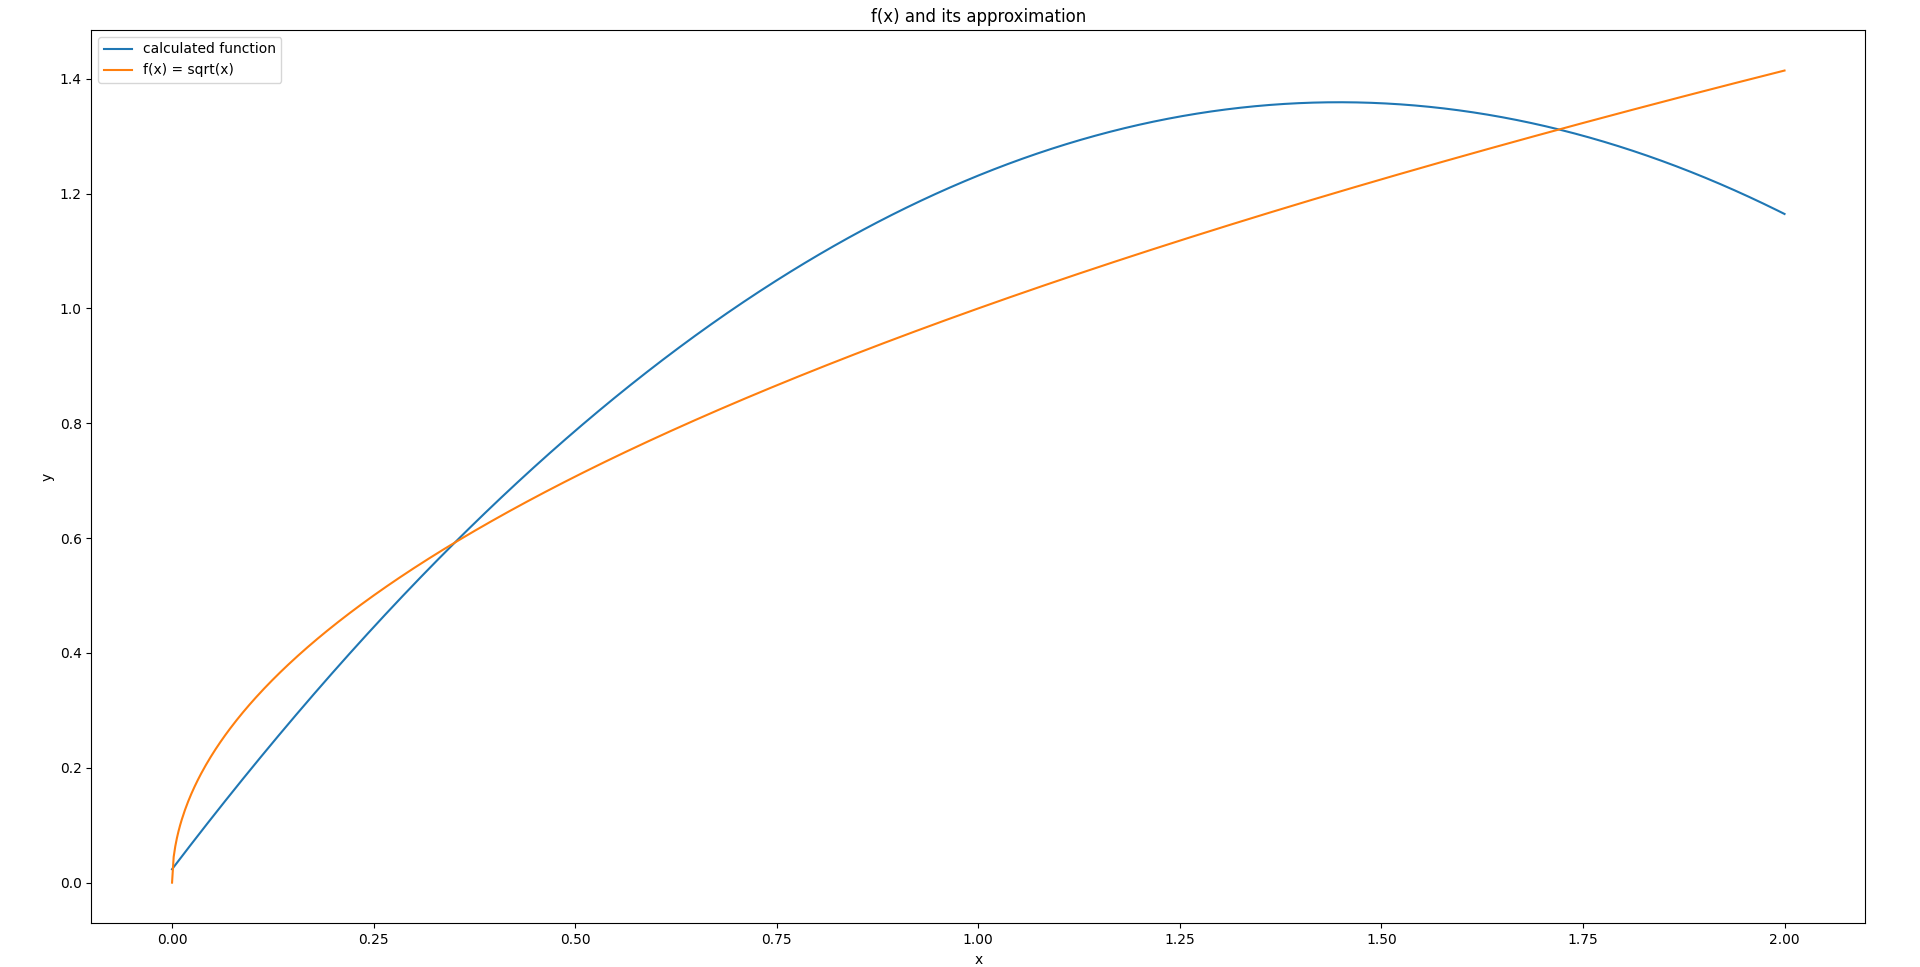
\includegraphics[scale = 0.3]{wykres2.png}
	\end{figure}
	
	
	
	
	
	
	
	
	
	
	
	
	
	
	
	
	
	
	
	
	
	
	
	
	
	
	
	
	
	
	
\end{document}